\documentclass[a4paper]{article}
\usepackage[T1]{fontenc}			% pacchetto per \chapter
\usepackage[italian]{babel}
\usepackage[italian]{isodate}  		% formato delle date in italiano
\usepackage{graphicx}				% gestione delle immagini
\usepackage{amsfonts}
\usepackage{booktabs}				% tabelle di qualità superiore
\usepackage{amsmath}				% pacchetto matematica
\usepackage{mathtools}				% per sottolineare sotto le equazioni
\usepackage{stmaryrd} 				% per '\llbracket' e '\rrbracket'
\usepackage{amsthm}					% teoremi migliorati
\usepackage{enumitem}				% gestione delle liste
\usepackage{pifont}					% pacchetto con elenchi carini
\usepackage{enumitem}				% pacchetto per elenchi con lettere dell'alfabeto
\usepackage{cancel}					% per cancellare delle espressioni matematiche
\usepackage{listings}				% implementa codice di programmazione


\usepackage[x11names]{xcolor}		% pacchetto colori RGB
% Link ipertestuali per l'indice
\usepackage{xcolor}
\usepackage[linkcolor=black, citecolor=blue, urlcolor=cyan]{hyperref}
\hypersetup{
	colorlinks=true
}

% Colour code style
\definecolor{codegreen}{rgb}{0,0.6,0}
\definecolor{codegray}{rgb}{0.5,0.5,0.5}
\definecolor{codepurple}{rgb}{0.58,0,0.82}
\definecolor{backcolour}{rgb}{0.95,0.95,0.92}

\lstdefinestyle{MATLAB}{
	backgroundcolor=\color{backcolour},   
	commentstyle=\color{codegreen},
	keywordstyle=\color{magenta},
	numberstyle=\tiny\color{codegray},
	stringstyle=\color{codepurple},
	basicstyle=\ttfamily\footnotesize,
	breakatwhitespace=false,         
	breaklines=true,                 
	captionpos=b,                    
	keepspaces=true,                 
	numbers=left,                    
	numbersep=5pt,
	showspaces=false,                
	showstringspaces=false,
	showtabs=false,                  
	tabsize=2
}
\lstset{style=MATLAB}

%\usepackage{showframe}				% visualizzazione bordi
%\usepackage{showkeys}				% visualizzazione etichetta

\newtheorem{theorem}{\textcolor{Red3}{\underline{Teorema}}}
\newtheorem{lemma}{Lemma}
\renewcommand{\qedsymbol}{QED}
\newcommand{\exec}[1]{\llbracket #1\:\rrbracket}
\newcommand{\dquotes}[1]{``#1''}
\newcommand{\longline}{\noindent\rule{\textwidth}{0.4pt}}

\begin{document}
	\author{Università degli Studi di Verona}
	\title{Simulazione di Elaborazione di segnali e immagini}
	\date{{\Large 15 Gennaio 2021}}
	\maketitle
	
	\section{Esercizio}
	
	Siano $x\left(t\right)$ e $y\left(t\right)$ due segnali di durata indefinita i cui spettri analitici $X\left(\mu\right)$ e $Y\left(\mu\right)$ sono rappresentati in figura 1 e figura 2 rispettivamente.
	\begin{figure}[!htp]
		\centering
		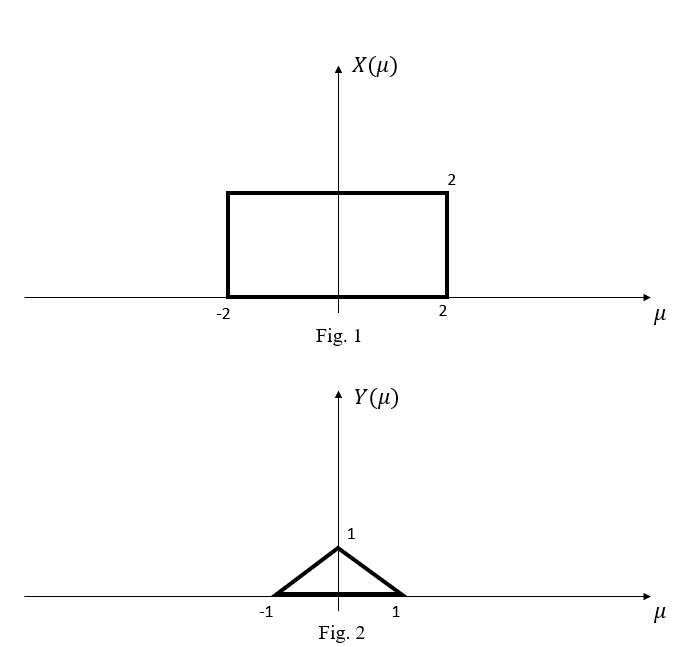
\includegraphics[width=\textwidth]{img/fig_1.png}
	\end{figure}

	\noindent
	Descrivere analiticamente, nel \underline{tempo} ed in \underline{frequenza} i segnali $X\left(\mu\right)$ ed $Y\left(\mu\right)$.\newpage
	
	\noindent
	Inoltre, descrivere analiticamente e graficamente, in \underline{frequenza}, i segnali $a\left(t\right)$, $b\left(t\right)$, $c\left(t\right)$, $d\left(t\right)$, $e\left(t\right)$ ottenuti come descritto nel sistema in figura 3.
	\begin{figure}[!htp]
		\centering
		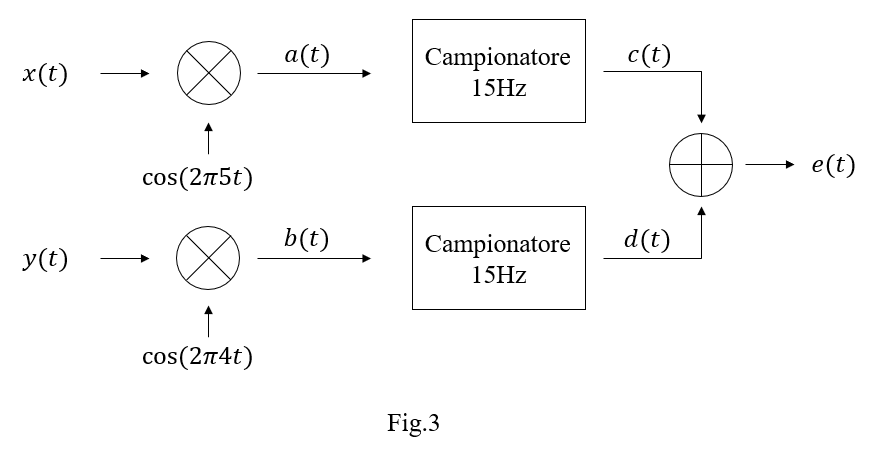
\includegraphics[width=\textwidth]{img/fig_2.png}
	\end{figure}

	\section{Esercizio}
	
	Sia $g\left(t\right)$ un segnale di durata indefinita la cui funzione nel tempo è definita come:
	\begin{equation*}
		g\left(t\right) = 20\mathrm{sinc}\left(10t\right) + 30\mathrm{sinc}\left(30t\right) e^{-j2\pi45t} + 30\mathrm{sinc}\left(30t\right) e^{j2\pi45t}
	\end{equation*}
	Descrivere analiticamente e graficamente, in frequenza, il segnale $G\left(\mu\right)$.\newline
	
	\noindent
	Inoltre, descrivere:
	\begin{itemize}
		\item Analiticamente, in frequenza e nel tempo
		\item Graficamente, in frequenza
	\end{itemize}
	Le elaborazioni a cui il segnale $g\left(t\right)$ è sottoposto se ad esso vengono applicate in sequenza le operazioni schematizzate nel sistema sottostante.
	\begin{figure}[!htp]
		\centering
		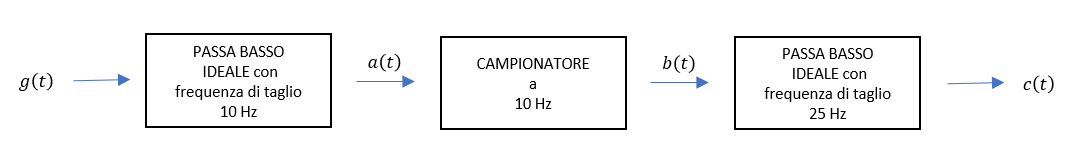
\includegraphics[width=\textwidth]{img/fig_3.png}
	\end{figure}\newpage

	\section{Esercizio}
	
	Siano $x\left(t\right)$ e $h\left(t\right)$ i due segnali nel dominio continuo del tempo raffigurati in figura 4.
	\begin{figure}[!htp]
		\centering
		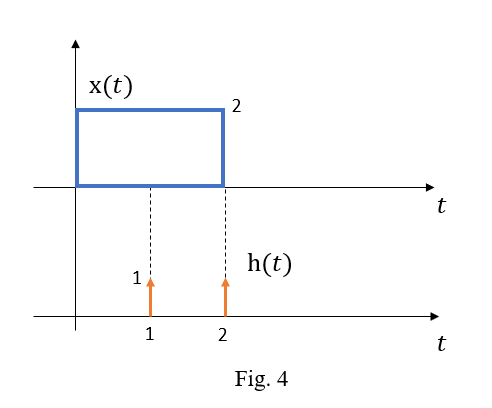
\includegraphics[width=.7\textwidth]{img/fig_4.png}
	\end{figure}
	
	\begin{itemize}
		\item Si descriva analiticamente e graficamente il segnale $y\left(t\right)$ ottenuto eseguendo la convoluzione $y\left(t\right) = x\left(t\right) * h\left(t\right)$;

		\item Si raffiguri graficamente il segnale $w\left(t\right) = \Pi\left(\frac{t - 1.5}{3}\right) - y\left(t\right)$
	\end{itemize}
	Facendo attenzione in entrambi i casi ad indicare attentamente tempo di inizio e fine del segnale, e il suo sviluppo nelle ordinate.
	
	\section{Esercizio}
	
	Eseguire l'operazione di equalizzazione della seguente matrice $4 \times 4$:
	\begin{table}[!htbp]
		\centering
		\begin{tabular}{@{} c | c | c | c @{}}
			\toprule
			0 & 0 & 1 & 3 \\
			1 & 0 & 4 & 5 \\
			7 & 2 & 0 & 6 \\
			7 & 4 & 7 & 7 \\
			\bottomrule
		\end{tabular}
	\end{table}
\end{document}